Using IB calculus, plus some vectors, we will be able to represent the motion of an object near a Lagrange point using equations.
It is important, however, that we first establish the system that we will be working with as well as restrictions that will make the mathematics slightly easier.
\begin{wrapfigure}{l}{0.6\textwidth}
	\centering
	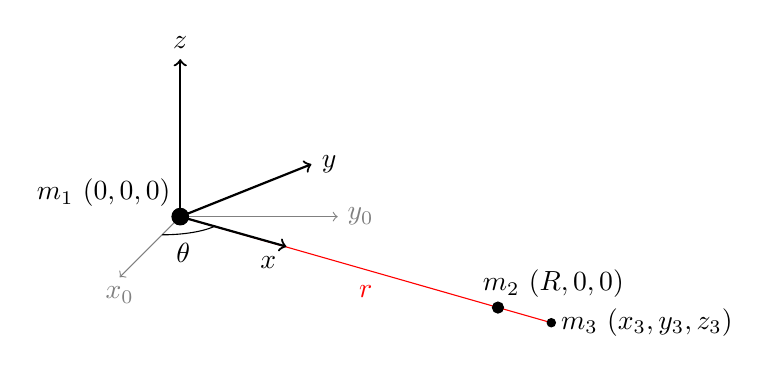
\begin{tikzpicture}
		\coordinate (o) at (0,0,0);
		\draw[thin,gray,->] (0,0,0) -- (0,0,2) node[below] {$\uvec{x}_0$};
		\draw[thin,gray,->] (0,0,0) -- (2,0,0) node[right] {$\uvec{y}_0$};
		
		\draw[red] (o) -- (6.06,0,3.5) node[midway,yshift=-8pt]{$\bvec{r}$};
		
		\draw[thick,->] (0,0,0) -- (0,2,0) node[above] {$\uvec{z}$};
		\draw[thick,->] (0,0,0) -- (1.73,0,0.99) node[below left] {$\uvec{x}$};
		\draw[thick,->] (0,0,0) -- (1,0,-1.73) node[right] {$\uvec{y}$};
		
		\draw (0,0,0.6) arc [start angle=-90,end angle=-32,x radius=0.8,y radius=0.24];
		\node at (.5,0,1.2) {$\theta$};
		
		\filldraw (0,0,0) circle (3pt) node[above left] {$m_1$ $(0,0,0)$};
		\filldraw (5.19,0,3) circle (2pt) node[above,xshift=20pt] {$m_2$ $(R,0,0)$};
		\filldraw (6.06,0,3.5) circle (1.5pt) node[right] {$m_3$ $(x_3,y_3,z_3)$};
	\end{tikzpicture}
	\vspace*{0.25cm}
	\caption{three-dimensional diagram of the Sun-Earth system with unit vectors relative to the Earth's orbit. Not drawn to scale.}
	\label{fig:3d-coords}
\end{wrapfigure}
Firstly, we must assert that $m_1 > m_2$, allowing the movement of the Sun due to the gravity of Earth is negligible.
This allows the Sun to be placed at the center of the coordinate system, avoiding the need to make considerations for the center of mass of the system.
It is also asserted that $m_2 > m_3$, so that, similarly to the previous assertion, the satellite has a negligible effect on Earth.
Secondly, continuing with the conditions from the previous calculations, it is assumed that the Earth is in a circular orbit, making the system a little easier to comprehend.
Thirdly, we assume that the orbit of the Earth has no inclination, meaning that it is on the same plane as $\uvec{x}$ and $\uvec{y}$.
Lastly, and as shown in Figure \ref{fig:3d-coords}, we will have basis vectors $\uvec{x}$, $\uvec{y}$, and $\uvec{z}$ drawn relative to the orbit of the Earth, with initial vectors $\uvec{x}_0$, $\uvec{y}_0$, and $\uvec{z}_0$.
The satellite around L2, $m_3$, will have the coordinates $(x_3,y_3,z_3)$ represented by the vector $\bvec{r}$.

It is also important to acknowledge that we will need to take the derivative of vectors. Hence, let us assert that, for some vector \textbf{v} with the basis vectors $\uvec{i}$ and $\uvec{j}$ scalars $a$ and $b$:
\begin{equation*}
	\frac{d}{dt}\bvec{v} = \frac{da}{dt}\uvec{i} + \frac{db}{dt}\uvec{j}
\end{equation*}
In other words, the derivative of a vector is equivalent to the derivative of its components.
This will allow us to analyze the movement of an object through kinematics in all three dimensions $x$, $y$, and $z$.

\newpage

One last thing: because we are dealing with vectors, Newton's law of gravitation can be rewritten in vector form:
\begin{equation*}
	\bvec{F} = \frac{Gm_1m_2}{r^3}\bvec{r}
\end{equation*}
where $r$ is the magnitude of $\bvec{r}$.

To start off, let us analyze our basis vectors. Because they are not actually static in the system ($\uvec{x}$ and $\uvec{y}$ rotate about the origin), their movement must be taken into account:
\begin{gather*}
	\uvec{x} = (\cos\theta)\uvec{x}_0 + (\sin\theta)\uvec{y}_0 \\
	\uvec{y} = -(\sin\theta)\uvec{x}_0 + (\cos\theta)\uvec{y}_0 \\
	\uvec{z} = \uvec{z}_0 \text{.}
\end{gather*}
Taking their first derivatives, we get:
\begin{gather*}
	\uvec{x}' = -(\sin\theta)\theta'\uvec{x}_0 + (\cos\theta)\theta'\uvec{y}_0 = \theta'\uvec{y} \\
	\uvec{y}' = -(\cos\theta)\theta'\uvec{x}_0 + (-\sin\theta)\theta'\uvec{y}_0 = -\theta'\uvec{x} \\
	\uvec{z}' = 0 \text{.}
\end{gather*}
And their second derivatives:
\begin{gather*}
	\uvec{x}'' = \theta''\uvec{y} + \theta'\uvec{y}' = \theta''\uvec{y} - \theta'^2\uvec{x} \\
	\uvec{y}'' = \theta''\uvec{y} + \theta'\uvec{x}' = -\theta''\uvec{x} - \theta'^2\uvec{y} \text{.}
\end{gather*}
The position vector $r$ is expressed as:
\begin{equation*}
	\bvec{r} = x_3\uvec{x} + y_3\uvec{y} + z_3\uvec{z}
\end{equation*}
We can take the second derivative of our position vector $\bvec{r}$ to find the acceleration.
\begin{equation*}
	\bvec{a} = \bvec{r}'' = (x_3\uvec{x})'' + (y_3\uvec{y})'' + (z_3\uvec{z})''
\end{equation*}
Our acceleration vector is then expanded to:
\begin{equation*}
	\bvec{a} = x_3''\uvec{x} + 2x_3'\uvec{x}' + x_3\uvec{x}'' + y_3'\uvec{y} + 2y_3'\uvec{y}' + x_3\uvec{y}'' + z_3''\uvec{z} + 2z_3'\uvec{z}' + z_3\uvec{z}''
\end{equation*}
Substituting the derivatives of the basis vectors that we calculated earlier,
\begin{gather*}
		\bvec{a} = x_3''\uvec{x} + 2x_3'(\theta'\uvec{y}) + x_3(\theta''\uvec{y} - \theta'^2\uvec{x}) + y_3''\uvec{y} - 2y_3'(\theta'\uvec{x}) - x_3(\theta''\uvec{x} + \theta'\uvec{y}) + z_3''\uvec{z} \\
		\bvec{a} = (x_3'' - \theta'^2x_3 - 2y_3'\theta' - y_3\theta'')\uvec{x} + (y_3'' + 2x_3'\theta' - \theta'^2y_3 + x_3\theta'')\uvec{y} + z_3''\uvec{z}
\end{gather*}
